
\subsubsection{Polinomi con coefficienti discordi}
Si consideri il seguente polinomio
$$
p(s) = s^5 + 8s^4 + 17s^3 + 8s^2 -14s - 10
$$
La condizione necessaria non è soddisfatta, il polinomio non può rappresentare
un sistema asintoticamente stabile, esisteranno delle radici la cui parte reale
sarà maggiore o uguale a zero.
Si costruisce comunque la tabella di Routh per esercizio e per contare il
numero di radici positive.
\begin{table}[h]
$$
\begin{array}{c:c|ccc}
& 5 & 1 & 17 & -4 \\
p & 4 & 8 & 8 & -10 \\ \hline
p & 3 & 16 &-23/2 \\
p & 2 & 55/4 & -20 \\
p & 1 & 259/22 \\
c & 0 & -20
\end{array}
$$
\end{table}
Sono presenti quattro permanenze di segno consecutive mentre il passaggio dalla
riga 1 alla riga 0 contiene una variazione di segno. Il polinomio avrà una sola
radice a parte reale positiva, la presenza del termine noto -10 esclude la
presenza di uno zero a parte reale nulla.
Risolvendo il polinomio con un calcolatore si ottiene:
$$
\lambda_i = \{ -5,-2,-1\pm j,1 \}
$$

\subsubsection{Ulteriore esempio}
Anche in questo caso non è soddisfatta la condizione necessaria
$$
p(s) = s^4 - 6s^3 - 11s^2 + 74 s + 78
$$
Si applica la tabella di Routh
$$
\begin{array}{c:c|ccc}
&4 & 1 & -11 & 78\\
c&3 & -6 & 74 \\ \hline
c&2 & 4/3 & 78 \\
p&1 & 425 \\
p&0 & 78
\end{array}
$$
Il polinomio ha due radici a parte reale negativa e due a parte reale maggiore
o uguale a zero
$$
\lambda_i = \{-3,-1,5\pm j\}
$$

\newpage
\subsubsection{Tabella contenente uno zero}
Si analizza il seguente polinomio
$$
p(s) = s^4 + s^3 + s^2 + s + 2
$$
È soddisfatta la condizione necessaria ma nella costruzione della tabella
compare uno zero, dunque non è ben definita e il polinomio non ammette tutte le
soluzioni a parte reale negativa.
$$
\begin{array}{c:c|cccc}
 & 4 & 1 & 1 & 2 \\
 & 3 & 1 & 1 \\ \hline
 & 2 & 0  \\
 & 1 \\
 & 0
\end{array}
$$

Se si volesse comunque contare il numero di zeri a parte reale positiva e
negativa esistono alcune tecniche equivalenti per continuare il calcolo.

\textbf{Tecnica delle perturbazioni elementari}

Si può sommare una $\varepsilon$ infinitesima positiva ai coefficienti, ossia
perturbarli localmente per eliminare lo zero, si continua lo sviluppo della
tabella:
$$
\begin{array}{cc:c|cccc}
\varepsilon<0 & \varepsilon>0  & 4 & 1 & 1 & 2 \\
p & p & 3 & 1 & 1 \\ \hline
c & p & 2 & \varepsilon & 2  \\
c & c & 1 & -2/\varepsilon\\
p & c & 0 & 2
\end{array}
$$
Il primo elemento sotto lo zero sarà
$$
c_{1,1} = -\frac{1}{\varepsilon}\begin{vmatrix}
1 & 1 \\
\varepsilon & 2
\end{vmatrix} = -\frac{1}{\varepsilon}(2-\varepsilon) \simeq
-\frac{2}{\varepsilon}
$$
Con $\varepsilon$ infinitesimo positivo si hanno due permanenze e due cambi di
segno, se $\varepsilon$ fosse negativo invece si vede che il risultato non
cambia.
Questa tecnica è valida se si azzera un elemento in prima colonna ma non
più di uno zero per riga.

\newpage
\subsubsection{Zeri multipli sulla stessa riga}
Si consideri una riga $i$-esima contenente più di uno zero tra i primi $p$
elementi, si moltiplicano i coefficienti della riga per $(-1)^p$,
successivamente si trasla la riga verso sinistra di $p$ posizioni eliminando
gli zeri, si somma questa nuova riga più piccola ottenuta e la si somma alla
riga $i$-esima originale; il risultato della somma viene sostituito al posto
della riga $i$-esima.


Si applica la tecnica al polinomio precedente, si vede che $p=1$, la riga 2
$(0,\ 2)$ viene moltiplicata per $-1$ e traslata di una posizione a sinistra
ottenendo $(-2,\ 0)$, successivamente sommata alla riga iniziale, si ottiene la
nuova tabella
$$
\begin{array}{c:c|cccc}
   & 4 & 1 & 1 & 2 \\
 p & 3 & 1 & 1 \\ \hline
 c & 2 & -2 & 2  \\
 c & 1 & 2 \\
 p & 0 & 2
\end{array}
$$

Un'ulteriore tecnica prevede di moltiplicare il polinomio per una radice nota,
aumentandone il grado, si ricostruisce la tabella di Routh, non dovrebbe
comparire più lo zero nella prima colonna, salvo casi eccezionali, se ciò non
dovesse accadere si può cambiare il valore della radice. Si dovrà togliere
successivamente al numero di radici positive o negative quella aggiunta
arbitrariamente, in base al suo segno.

\subsubsection{Annullamento di un'intera riga}
Si consideri il polinomio
$$
p(s) = s^5 + s^4 + s^3 + s^2 + s + 1
$$
La condizione necessaria è verificata, si costruisce la tabella di Routh, tutta
la riga 3 sarà nulla
$$
\begin{array}{c:c|ccc}
  & 5 & 1 & 1 & 1 \\
p & 4 & 1 & 1 & 1 \\ \hline
  & 3 & 0 & 0 \\
  & 2 \\
  & 1 \\
  & 0
\end{array}
$$
In questo caso il polinomio di partenza può essere fattorizzato in un prodotto
di due polinomi $p'(s) \cdot p''(s)$, il primo polinomio dipende da tutte le
righe della tabella di Routh fino a quella prima della riga nulla, in questo
caso 5 e 4. Un'intera riga si può annullare solo in posizioni dispari (3).
Le radici contenute nel polinomio $p'$ rispettano la permanenza di segno delle
righe precedenti a quella annullata, di conseguenza in questo caso il polinomio
$p'$ avrà una sola radice con parte reale negativa.
Le restanti righe riguardano il polinomio $p''$, sarà di ordine pari al numero
di righe rimanenti, è di ordine sempre pari ed è biquadratico, ossia scrivibile
nella forma $s^2$.

Le radici di un polinomio biquadratico hanno sempre simmetria quadrantale, una
radice reale avrà una radice simmetrica sull'asse reale di segno opposto, una
coppia di radici complesse e coniugate avranno un'altra coppia sul lato opposto
rispetto all'asse reale; ogni quadrante ha la stessa disposizione delle
radici, si ottiene ruotando quello adiacente.

Sicuramente la condizione necessaria di Routh non è soddisfatta, avrà solo i
coefficienti delle potenze pari mentre quelli delle potenze dispari saranno
nulli, in ogni caso non potrebbero esistere radici che non appartengano almeno
all'asse immaginario o siano a parte reale positiva.

I coefficienti del polinomio $p''$ sono quelli dell'ultima riga prima prima
della riga nulla
$$
p''(s) = s^4 + s^2 + 1
$$
Si potrebbe ottenere il polinomio $p'$ eseguendo una divisione
$$
\polylongdiv[style=D,vars=s]{s^5+s^4+s^3+s^2+s+1}{s^4+s^2+1}
$$
Più rapidamente si può ottenere la riga mancante in tabella derivando il
polinomio $p''$ ed inserendo i coefficienti ottenuti $\frac{dp''(s)}{ds} = 4s^3
+ 2s$.

La nuova tabella ottenuta sarà
$$
\begin{array}{c:c|ccc}
  & 5 & 1 & 1 & 1 \\
p & 4 & 1 & 1 & 1 \\ \hline
p & 3 & 4 & 2 & \frac{dp''}{ds}\\
p & 2 & 2 & 4 &(\times 4)\\
c & 1 & -12 & & (\times2)\\
c & 0 & 4
\end{array}
$$
Il polinomio $p''$ avrà due radici a parte reale negativa e due a parte
reale positiva.

\newpage
\subsection{Studio dei sistemi a parametri incerti}
Un sistema è a parametri incerti se alcuni suoi parametri sono forniti con un
intervallo di incertezza oppure non sono ancora stati dimensionati, ad esempio
il sistema può contenere dei regolatori a struttura preassegnata come i
regolatori ``PID'' (\textit{Proporzionali-Integrali-Derivativi}) la cui
struttura e consecutiva legge di controllo sono già assegnati, vanno solo
impostati i giusti parametri.
Si cerca dunque la regione di asintotica stabilità (RAS) nell'insieme dei
parametri, il criterio di Routh si presta bene a questi studi.

Si consideri il polinomio
$$
p(s) =s^3 + (2+\beta)^2s^2 + (1+2\beta)s + \alpha + \beta \qquad \alpha,\beta
\in \mathbb{R}
$$

Si deve sempre imporre la condizione necessaria
$$\left\{\begin{aligned}
2+\beta &> 0 \\
1+2\beta &> 0 \\
\alpha+ \beta &> 0
\end{aligned}\right.\Rightarrow
\left\{\begin{aligned}
&\cancel{\beta  > -2}\\
&\beta  > -\frac{1}{2} \\
&\beta  > -\alpha
\end{aligned}\right.
$$
Con soli due parametri è possibile rappresentare graficamente questa regione,
la RAS è sicuramente contenuta in questa regione, potrebbe essere però più
piccola. Per individuare la RAS si costruisce la tabella di Routh, i
coefficienti della prima colonna devono avere tutti lo stesso segno
$$
\begin{array}{c|cc}
3 & 1 & 1+2\beta \\
2 & 2+\beta & \alpha + \beta \\ \hline
1 & \frac{2(\beta+1)^2-\alpha}{2+\beta}\\
0 & \alpha+\beta
\end{array}\Rightarrow\left\{
\begin{aligned}
&2+\beta > 0 \\
&\frac{2(\beta+1)^2-\alpha}{2+\beta} > 0\\
&\alpha + \beta > 0
\end{aligned}\right.\Rightarrow
\left\{\begin{aligned}
&\beta>-2\\
&2(\beta+1)^2 > \alpha\\
&\beta > -\alpha
\end{aligned}\right.
$$
Intersecando i due sistemi ottenuti si ottiene la RAS
\begin{figure}[h]
 \centering
 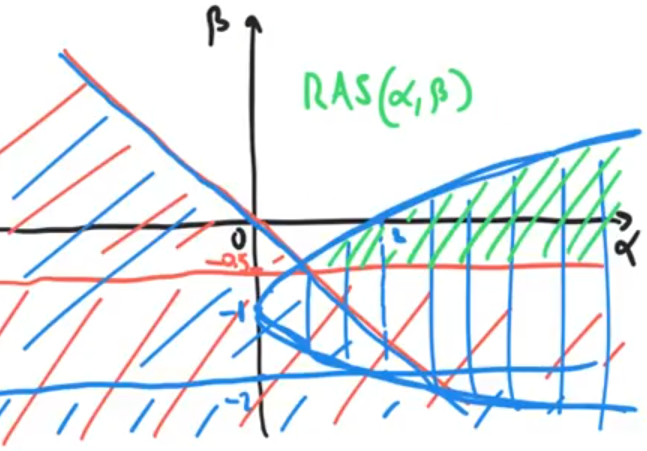
\includegraphics[width=\picwid]{ras_alpha_beta}
\end{figure}

\newpage
\subsubsection{Criterio di Karithonov}
Il criterio di Karithonov fa uso del criterio di Routh per risolvere il
problema di un sistema definito da parametri con una certa tolleranza.

Si consideri un polinomio definito dalla seguente lista di coefficienti
compresi in un certo intervallo di valori:
$$
p(s) : \{\alpha_0,\alpha_1,\alpha_2,\ldots,\alpha_n\} \qquad
\alpha_i\in[\alpha_i^-,\alpha_i^+]\quad i=0,\ldots,n
$$

È un caso tipico di tutti i sistemi i cui parametri sono forniti dal
costruttore con una tolleranza oppure sono stati studiati mediante un certo
strumento con un'accuratezza finita o ancora sono sottoposti a temperature
molto diverse tra loro e i loro parametri hanno una certa dipendenza dalla
temperatura.

Al fine di studiare l'asintotica stabilità vengono costruiti quattro polinomi
utilizzando gli estremi di ogni parametro secondo uno specifico ordine
$$
\begin{aligned}
P_a(s) &:
\{\alpha_0^+,\alpha_1^+,\alpha_2^-,\alpha_3^-,\alpha_4^+,\alpha_5^+,\ldots\}\\
P_b(s) &:
\{\alpha_0^-,\alpha_1^-,\alpha_2^+,\alpha_3^+,\alpha_4^-,\alpha_5^-,\ldots\}\\
P_c(s) &:
\{\alpha_0^+,\alpha_1^-,\alpha_2^-,\alpha_3^+,\alpha_4^+,\alpha_5^-,\ldots\}\\
P_d(s) &:
\{\alpha_0^-,\alpha_1^+,\alpha_2^+,\alpha_3^-,\alpha_4^-,\alpha_5^+,\ldots\}
\end{aligned}
$$
Il polinomio $P_b$ è il negato di $P_a$, il polinomio $P_c$ ha i segni traslati
di una posizione verso sinistra rispetto a $P_a$, il polinomio $P_c$ è il
negato di $P_a$.

1:02:31
